\begin{figure}[h!]
	\centering
	
	
	
	\tikzset{every picture/.style={line width=0.75pt}} %set default line width to 0.75pt        
	
	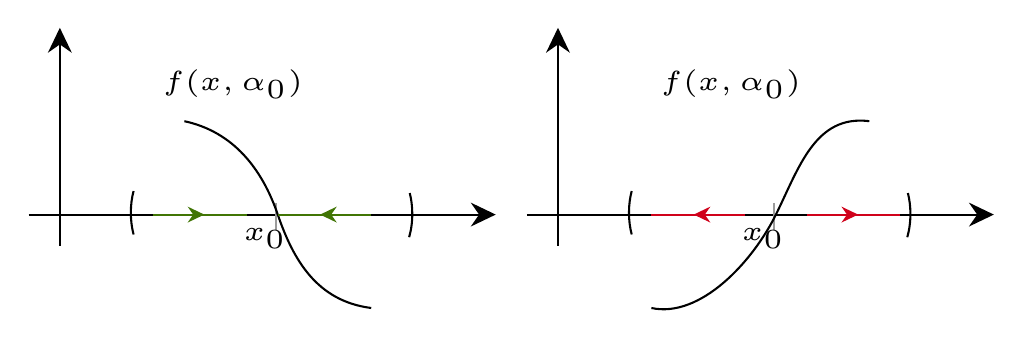
\begin{tikzpicture}[x=0.75pt,y=0.75pt,yscale=-1.5,xscale=1.5]
		%uncomment if require: \path (0,300); %set diagram left start at 0, and has height of 300
		
		%Straight Lines [id:da6141249148083039] 
		\draw    (80,150) -- (227,150) ;
		\draw [shift={(230,150)}, rotate = 180] [fill={rgb, 255:red, 0; green, 0; blue, 0 }  ][line width=0.08]  [draw opacity=0] (8.04,-3.86) -- (0,0) -- (8.04,3.86) -- (5.34,0) -- cycle    ;
		%Straight Lines [id:da4256457462457566] 
		\draw    (90,160) -- (90,93) ;
		\draw [shift={(90,90)}, rotate = 90] [fill={rgb, 255:red, 0; green, 0; blue, 0 }  ][line width=0.08]  [draw opacity=0] (8.04,-3.86) -- (0,0) -- (8.04,3.86) -- (5.34,0) -- cycle    ;
		%Shape: Arc [id:dp06425887483981807] 
		\draw  [draw opacity=0] (113.68,156.39) .. controls (113.12,154.26) and (112.8,151.89) .. (112.8,149.4) .. controls (112.8,146.92) and (113.11,144.56) .. (113.68,142.43) -- (122.8,149.4) -- cycle ; \draw   (113.68,156.39) .. controls (113.12,154.26) and (112.8,151.89) .. (112.8,149.4) .. controls (112.8,146.92) and (113.11,144.56) .. (113.68,142.43) ;  
		%Shape: Arc [id:dp36365112063998306] 
		\draw  [draw opacity=0] (202.39,143.08) .. controls (202.91,145.14) and (203.2,147.41) .. (203.2,149.8) .. controls (203.2,152.48) and (202.84,155.01) .. (202.19,157.26) -- (193.2,149.8) -- cycle ; \draw   (202.39,143.08) .. controls (202.91,145.14) and (203.2,147.41) .. (203.2,149.8) .. controls (203.2,152.48) and (202.84,155.01) .. (202.19,157.26) ;  
		%Straight Lines [id:da9959510519703285] 
		\draw [color={rgb, 255:red, 155; green, 155; blue, 155 }  ,draw opacity=1 ]   (159.4,146.2) -- (159.4,155) ;
		%Curve Lines [id:da23263506141610102] 
		\draw    (130,120) .. controls (145.8,123.4) and (155,135.4) .. (160,150) .. controls (165,164.6) and (172.6,177.8) .. (190,180) ;
		%Straight Lines [id:da06316055058145875] 
		\draw [color={rgb, 255:red, 65; green, 117; blue, 5 }  ,draw opacity=1 ]   (120,150) -- (150,150) ;
		\draw [shift={(136.4,150)}, rotate = 180] [fill={rgb, 255:red, 65; green, 117; blue, 5 }  ,fill opacity=1 ][line width=0.08]  [draw opacity=0] (5.36,-2.57) -- (0,0) -- (5.36,2.57) -- (3.56,0) -- cycle    ;
		%Straight Lines [id:da5497631725058023] 
		\draw [color={rgb, 255:red, 65; green, 117; blue, 5 }  ,draw opacity=1 ]   (190,150) -- (160,150) ;
		\draw [shift={(173.6,150)}, rotate = 360] [fill={rgb, 255:red, 65; green, 117; blue, 5 }  ,fill opacity=1 ][line width=0.08]  [draw opacity=0] (5.36,-2.57) -- (0,0) -- (5.36,2.57) -- (3.56,0) -- cycle    ;
		%Straight Lines [id:da09861653689071792] 
		\draw    (240,150) -- (387,150) ;
		\draw [shift={(390,150)}, rotate = 180] [fill={rgb, 255:red, 0; green, 0; blue, 0 }  ][line width=0.08]  [draw opacity=0] (8.04,-3.86) -- (0,0) -- (8.04,3.86) -- (5.34,0) -- cycle    ;
		%Straight Lines [id:da21639286510164335] 
		\draw    (250,160) -- (250,93) ;
		\draw [shift={(250,90)}, rotate = 90] [fill={rgb, 255:red, 0; green, 0; blue, 0 }  ][line width=0.08]  [draw opacity=0] (8.04,-3.86) -- (0,0) -- (8.04,3.86) -- (5.34,0) -- cycle    ;
		%Shape: Arc [id:dp8981115574458696] 
		\draw  [draw opacity=0] (273.68,156.39) .. controls (273.12,154.26) and (272.8,151.89) .. (272.8,149.4) .. controls (272.8,146.92) and (273.11,144.56) .. (273.68,142.43) -- (282.8,149.4) -- cycle ; \draw   (273.68,156.39) .. controls (273.12,154.26) and (272.8,151.89) .. (272.8,149.4) .. controls (272.8,146.92) and (273.11,144.56) .. (273.68,142.43) ;  
		%Shape: Arc [id:dp06952342542904488] 
		\draw  [draw opacity=0] (362.39,143.08) .. controls (362.91,145.14) and (363.2,147.41) .. (363.2,149.8) .. controls (363.2,152.48) and (362.84,155.01) .. (362.19,157.26) -- (353.2,149.8) -- cycle ; \draw   (362.39,143.08) .. controls (362.91,145.14) and (363.2,147.41) .. (363.2,149.8) .. controls (363.2,152.48) and (362.84,155.01) .. (362.19,157.26) ;  
		%Straight Lines [id:da1271782911650352] 
		\draw [color={rgb, 255:red, 155; green, 155; blue, 155 }  ,draw opacity=1 ]   (319.4,146.2) -- (319.4,155) ;
		%Curve Lines [id:da20362079394350396] 
		\draw    (280,180) .. controls (295.8,183.4) and (312.6,165) .. (320,150) .. controls (327.4,135) and (332.6,117.8) .. (350,120) ;
		%Straight Lines [id:da6324765334271558] 
		\draw [color={rgb, 255:red, 208; green, 2; blue, 27 }  ,draw opacity=1 ]   (330,150) -- (360,150) ;
		\draw [shift={(346.4,150)}, rotate = 180] [fill={rgb, 255:red, 208; green, 2; blue, 27 }  ,fill opacity=1 ][line width=0.08]  [draw opacity=0] (5.36,-2.57) -- (0,0) -- (5.36,2.57) -- (3.56,0) -- cycle    ;
		%Straight Lines [id:da3762166451314517] 
		\draw [color={rgb, 255:red, 208; green, 2; blue, 27 }  ,draw opacity=1 ]   (310,150) -- (280,150) ;
		\draw [shift={(293.6,150)}, rotate = 360] [fill={rgb, 255:red, 208; green, 2; blue, 27 }  ,fill opacity=1 ][line width=0.08]  [draw opacity=0] (5.36,-2.57) -- (0,0) -- (5.36,2.57) -- (3.56,0) -- cycle    ;
		
		% Text Node
		\draw (121,101.4) node [anchor=north west][inner sep=0.75pt]  [font=\tiny,xscale=2,yscale=2]  {$f( x,\alpha _{0})$};
		% Text Node
		\draw (147,152.4) node [anchor=north west][inner sep=0.75pt]  [font=\tiny,xscale=2,yscale=2]  {$x_{0}$};
		% Text Node
		\draw (281,101.4) node [anchor=north west][inner sep=0.75pt]  [font=\tiny,xscale=2,yscale=2]  {$f( x,\alpha _{0})$};
		% Text Node
		\draw (307,152.4) node [anchor=north west][inner sep=0.75pt]  [font=\tiny,xscale=2,yscale=2]  {$x_{0}$};
		
		
	\end{tikzpicture}
\end{figure}